\section{Boosted decision trees}
\label{sec:BDT}

Boosted decision trees (BDT's) are one of the easiest ways to implement Machine Learning. It's typically not very sensitive to its parameters, and is relatively easy to set up. In this thesis we have used XGBoost \cite{xgboostAbout}, which is one specific way to boost a decision tree. Before we explain boosted DTs however, we have to understand a regular DT.


\subsection{Decision tree}

A decision tree is something we do when thinking quite often, even if we don't refer to the process as such. When we make a choice, we use a decision tree. Let us say that we have a picture of a person and we want to figure out if it is a boy or a girl. To make this conclusion we identify different features like whether the person has long hair, a beard, makeup, and so on. Then we set up a decision tree that will split our input data, which in this case is our picture, and make decisions based on the features you give it. Of course, we are not going to look on gender recognition in this thesis, but in principle decision trees can classify many things. This was just a small illustration of the simplicity and broad usage of BDT's.

Our goal is to use these principles to separate the signal from the background events. We give our decision tree some input data \cite{DTppt}, which consists of Monte Carlo (MC) simulated background and different signal samples (which are also obtained by MC simulations). Our decision tree will then split our data based on features we provide, e.g. invariant mass and missing transverse energy. 

\begin{figure}[H]
    \centering
    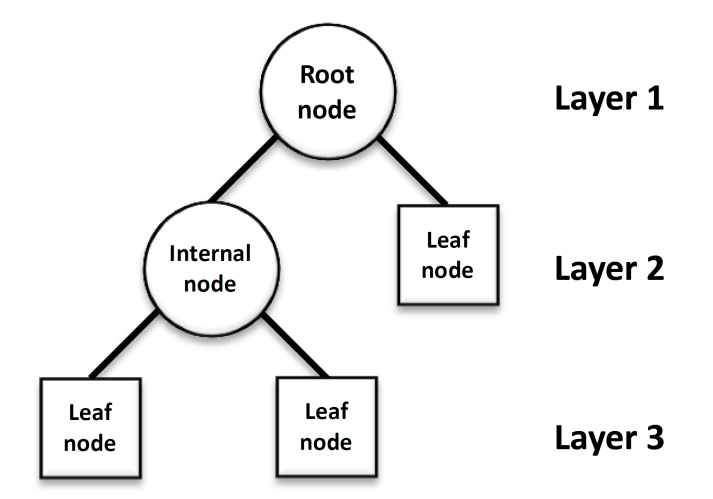
\includegraphics[width=0.5\textwidth]{Figures/FromOnline/Basic-structure-of-a-decision-tree-All-decision-trees-are-built-through-recursion.png}
    \caption{A sketch of how a decision tree is set up. \cite{DTpic}}
    \label{fig:DTpic}
\end{figure}

If we look at figure \ref{fig:DTpic}, we can see that we have three layers and three different types of nodes. The \textit{root node} is our input node, i.e. our input data, which for the first round is signal and background samples. Then the decision tree splits up our input data depending on what features we give it. This part will happen continuously through \textit{internal nodes} until we hit the depth of the tree, i.e. the last layer, or only have \textit{leaf nodes} left. As mentioned in section \ref{sec:TandT}, we split our input data into train and test parts where we save some data to test how well our model is trained. If we are happy with our results, we can test our pretrained model on real data and potentially extract some signal.


\subsection{Boosting}
Decision trees are weak learners (meaning that they typically perform badly), but if we ensemble several weak learners, we can get a strong learner. This process gives what it is called a boosted decision trees. Boosting creates a collection of predictors, which means that we fit consecutive trees, and at every step, we try to solve for the net error from the prior tree. If a hypothesis misclassifies the input, its weight will increase, so it would more likely classify it correctly next time. In figure \ref{fig:BDT}, we can see a sketched diagram of a BDT.


\begin{figure}[H]
    \centering
    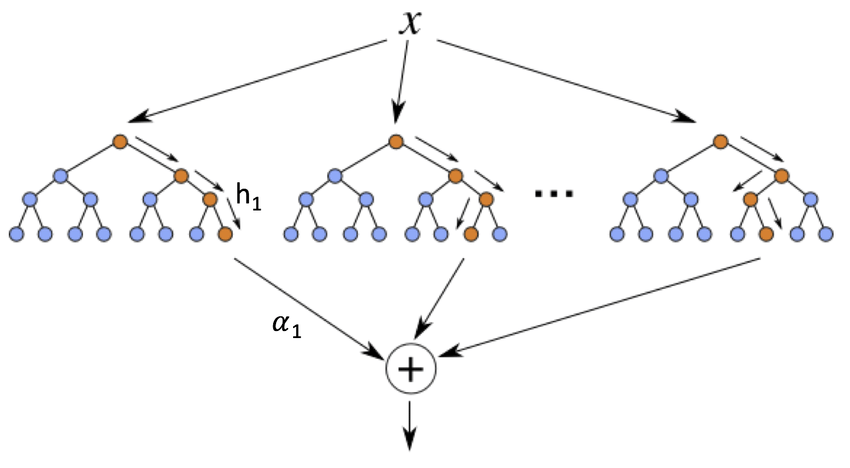
\includegraphics[width = 0.7\textwidth]{Figures/FromOnline/BDT.png}
    \caption{Illustration of a BDT \cite{BDTpic}.}
    \label{fig:BDT}
\end{figure}

There are many ways to boost a decision tree, but in this thesis we have used a Python software library called XGBoost \cite{xgboostAbout}, which is short for eXtreme Gradient Boosting. This library uses a gradient descent while boosting the decision trees. The gradient descent is an algorithm that can optimize the differentiable loss function, i.e., the next tree will try to recover the loss from the previous tree. Note that the loss is defined as the difference between actual and predicted values \cite{BDT}. 

XGBoost is optimized to be highly efficient and flexible \cite{xgboostAbout}. It is written in C++, but offers a user interface in python and other languages. In this thesis we are using a class in XGBoost called \texttt{XGBClassifier} which, as implied by the name, classifies the data. We give all our input data a label 0 or 1 for background and signal respectively and train our model, with the different features, on what should have label 0 or 1 in the end. This is what we call \textit{supervised learning} because we help our model by providing a label in the input. The \texttt{XGBClassifier} takes a lot of arguments, which can be found in the Scikit-Learn API reference guide \cite{xgboostargument}, but in this thesis we use just the ones that are necessary for our purpose. The arguments that we have used are mentioned in the analysis chapter.

\subsection{Feature importance}
We are also going to look at the feature importance in the analysis. This is a way to see which features were important while constructing our BDT. This is an interesting aspect of the analysis because this will change from process to process and we will also be able to see if it matters if we train on different signal samples or not.